\section{Declarative Programmable Storage}
\label{sec:prog-model}

Current ad-hoc approaches to programmable storage restrict use to developers
with distributed programming expertise, knowledge of the intricacies of the
underlying storage system and its performance model, and primarily use
hard-coded imperative methods. This restricts the use of optimizations that
can be performed automatically or derived from static analysis.  Based on the
challenges we have demonstrated stemming from the dynamic nature and large
design space of programmable storage, we present an alternative, declarative
programming model that can reduce the learning curve for new users, and allow
existing developers to increase productivity by writing less code that is more
portable.

The model we propose corresponds to a subset of the Bloom language which is a
declarative language for expressing distributed programs as an unordered set
of rules~\cite{alvaro:cidr11}. These rules fully specify program semantics and
allow a programmer to ignore the details associated with how a program is
evaluated. This level of abstraction is attractive for building storage
interfaces whose portability and correctness is critical. We model the
storage system state uniformly as a collection of relations, with interfaces
being expressed as a collection of \emph{queries} over a request stream that
are filtered, transformed, and combined with system state. Next we present a
brief example of the CORFU shared-log interface expressed using this model.

\subsection{Example: The CORFU Log Interface}

The CORFU log protocol achieves high-performance in part by striping the log
across a large number of fast storage devices. Using our declarative language
we model the log as a single relation, hiding the implementation detail of log
partitioning. Lines 2-3 in Listing~\ref{lst:corfublm} show the declaration of
state for the CORFU interface consisting of two persistent collections: one for
the log data, and one for interface metadata. The mapping of collections onto
physical storage is abstracted at this level, permitting optimizations
discussed earlier to be discovered and applied transparently by an optimizer.
Line 5 defines the write operation as a scratch collection with models
non-persistent state only valid for the duration of a single time stemp
allowing an optimizer to treat this state as volatile.

\begin{lstlisting}[caption={Sample \emph{corfu.bloom} program listing}, label=lst:corfublm]
bloom :corfu do
  table :epoch, [:epoch]
  table :log, [:pos] => [:state, :data]
  scratch :write_op, op.schema
end
bloom :write do
  temp :valid_write <= write_op.notin(found_op)
  log <+ valid_write{|o| [o.pos, 'ok', o.data]}
  ret <= valid_write{|o| [o.type, o.pos, o.epoch, 'ok'] }
  ret <= write_op.notin(valid_write) {|o| ['read-only'] }
end
bloom :trim do
  log <+- trim_op{|o| [o.pos, 'trimmed']}
  ret <=  trim_op{|o|
    [o.type, o.pos, o.epoch, 'ok']}
end
\end{lstlisting}

The write-once 64-bit address space exposed by CORFU storage devices depends on
a method for quickly resolving the log position to metadata and physical
storage addresses. The declarative specification of the write interface shown
on lines 8-13 is expressed independently of the implementation and any
optimization strategies.  In addition, the CORFU interface depends on a trim
interface to mark unused poritions of the log (shown on lines 10-15) Trimmed
entries are tracked as unused for reclamation, and implementations may take
advantage of specific optimizations provided by an index implementation or
hardware support found in modern non-volatile memories.

\begin{figure}
\centering
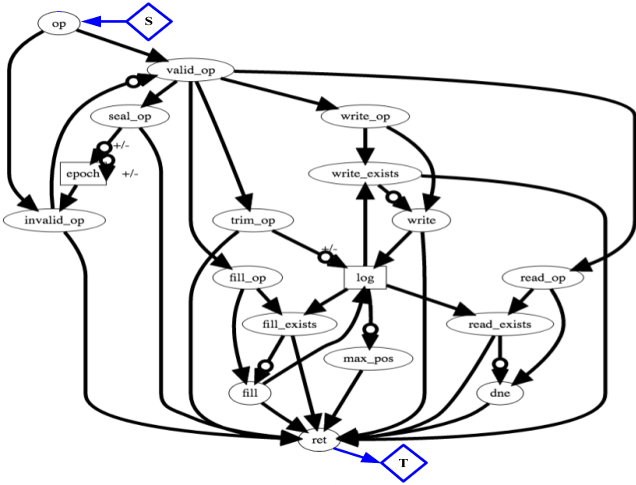
\includegraphics[width=0.7\columnwidth]{Corfu_viz_expanded2.png}
\caption{Dataflow graph for the CORFU interface written in Bloom}
\label{fig:flow}
\end{figure}

Amazingly, only a few code snippets can express the semantics of the entire
storage device interface requirements in CORFU\footnote{Due to space
limitations refer to \cite{watkins:ucsc-soe-16-12} for a full program
listing.}.  Figure~\ref{fig:flow} shows the dataflow diagram for the entire
CORFU program expressed in Bloom that can serve as input to an optimizer.
Beyond the convenience of writing less code, it is far easier for the
programmer writing an interface such as CORFU to convenience herself of the
correctness of the high-level details of the implementation without being
distracted by issues related to physical design or the many other gotchas that
one must deal with when writing low-level systems software.

%For reference our prototype implementation of CORFU in Ceph (called
%ZLog\footnote{https://github.com/noahdesu/zlog}) is written in C++ and the
%storage interface component comprises nearly 700 lines of code, and uses a
%hard-coded indexing strategy that has been rewritten multiple times to explore
%alternative optimization techniques.

%\begin{figure}[t]
%\begin{subfigure}{.2\columnwidth}
%\centering
%\scalebox{0.4}{
%\begin{tikzpicture}[->,>=stealth',shorten >=1pt,auto,node distance=2.2cm,semithick]
%%\tikzstyle{every state}=[fill=red,draw=none,text=white]
%
%  \node[initial left,state] (A)              {$EG$};
%  \node[state]         (B) [below right of=A] {$CP$};
%  \node[state]         (D) [right of=B]       {$IO$};
%  \node[state]         (C) [above right of=A] {$GC$};
%  \node[state]         (E) [right of=C]       {$US$};
%  \node[state]         (F) [below right of=E] {$Out$};
%
%  \path (A) edge        node [left] {R,W,F} (B)
%            edge        node {T}     (C)
%        (B) edge        node {F}     (C)
%            edge        node {R,W}   (D)
%        (C) edge        node {F,T}   (E)
%        (D) edge        node {W}     (E)
%            edge        node {R}     (F)
%        (E) edge        node {F,T,W} (F);
%\end{tikzpicture}
%}
%\caption{}
%\label{fig:corfu-sm}
%\end{subfigure}\hfill
%\begin{subfigure}{.6\columnwidth}
%\centering
%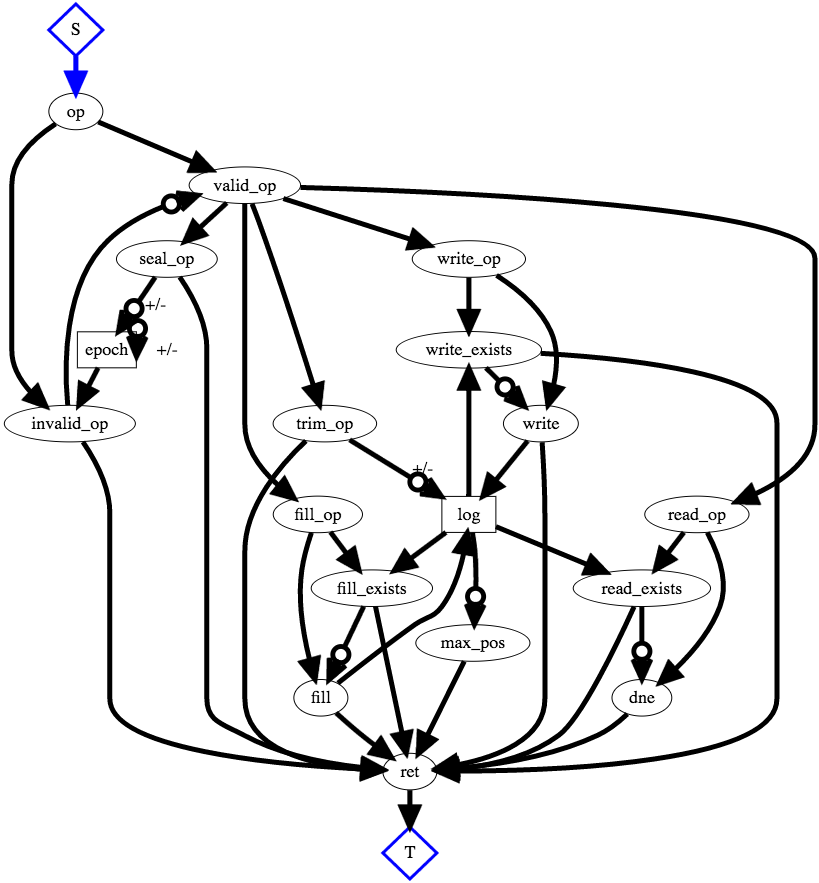
\includegraphics[width=1.0\columnwidth]{Corfu_viz_expanded.png}
%\caption{}
%\label{fig:malacologyx}
%\end{subfigure}
%\end{figure}

%\begin{figure*}[t]
%\begin{subfigure}{.3\columnwidth}
%\centering
%\scalebox{0.45}{
%\begin{tikzpicture}[->,>=stealth',shorten >=1pt,auto,node distance=2.2cm,semithick]
%%\tikzstyle{every state}=[fill=red,draw=none,text=white]
%
%  \node[initial left,state] (A)              {$EG$};
%  \node[state]         (B) [below right of=A] {$CP$};
%  \node[state]         (D) [right of=B]       {$IO$};
%  \node[state]         (C) [above right of=A] {$GC$};
%  \node[state]         (E) [right of=C]       {$US$};
%  \node[state]         (F) [below right of=E] {$Out$};
%
%  \path (A) edge        node [left] {R,W,F} (B)
%            edge        node {T}     (C)
%        (B) edge        node {F}     (C)
%            edge        node {R,W}   (D)
%        (C) edge        node {F,T}   (E)
%        (D) edge        node {W}     (E)
%            edge        node {R}     (F)
%        (E) edge        node {F,T,W} (F);
%\end{tikzpicture}
%}
%\caption{}
%\label{fig:corfu-sm}
%\end{subfigure}\hfill
%\begin{subfigure}{.5\columnwidth}
%\centering
%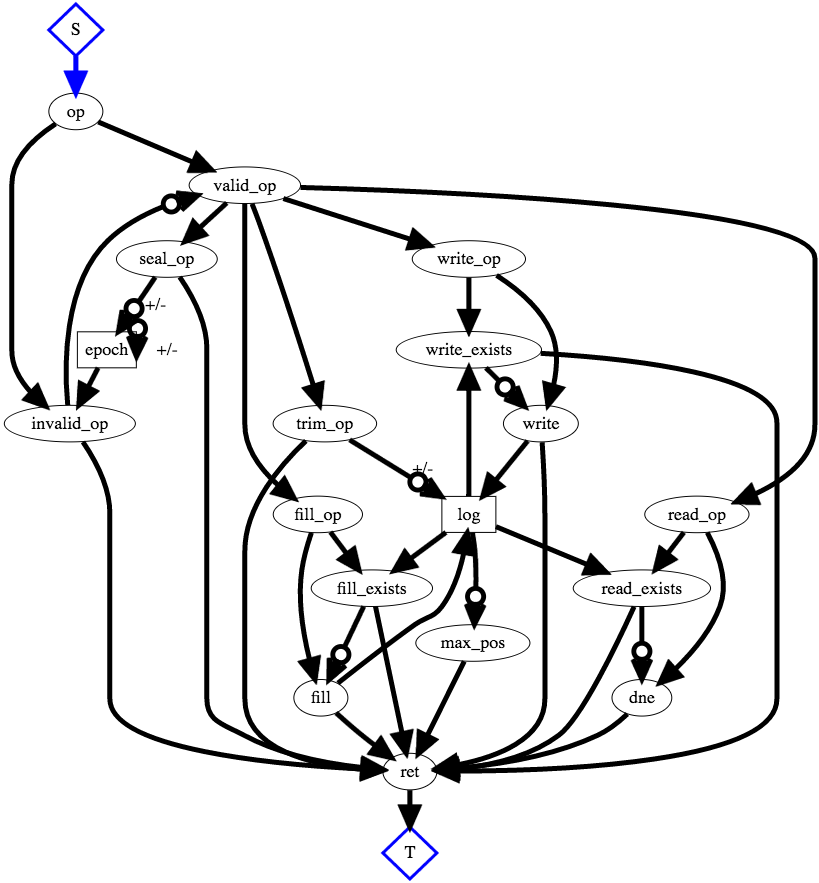
\includegraphics[width=0.95\columnwidth]{Corfu_viz_expanded.png}
%\caption{}
%\label{fig:malacologyx}
%\end{subfigure}\hfill
%\begin{subfigure}{0.9\columnwidth}
%
%\begin{lstlisting}[title={{\bf (c)}}, label=lst:write]
%bloom :write do
%  temp :valid_write <= write_op.notin(found_op)
%  log <+ valid_write{ |o| [o.pos, 'valid', o.data]}
%  ret <= valid_write{ |o|
%    [o.type, o.pos, o.epoch, 'ok'] }
%  ret <= write_op.notin(valid_write) {|o|
%    [o.type, o.pos, o.epoch, 'read-only'] }
%end
%\end{lstlisting}
%\end{subfigure}
%\caption{foo}
%\end{figure*}

